\newpage
\setcounter{section}{0}
\renewcommand{\thesection}{\arabic{section}}

\begin{center}
    \Huge
    \textbf{Modul 2}
    
    Wireless Connection

\end{center}


\section{pendahuluan}

Pada modul ini, kita akan membahas konfigurasi routing static dan routing dinamis pada perangkat
MikroTik. Routing merupakan proses pengiriman data antara dua atau lebih jaringan yang berbeda.

Dalam modul ini, kita akan membahas konsep dasar routing, macam-macam routing statis dan
dinamis, serta langkah-langkah untuk mengkonfigurasi kedua jenis routing ini pada perangkat
MikroTik.

Sebelum memulai pembahasan routing, penting untuk memahami konsep dasar jaringan dan
subnetting. Jaringan terdiri dari sejumlah perangkat yang terhubung satu sama lain, seperti komputer,
printer, dan perangkat jaringan lainnya. Setiap perangkat dalam jaringan memiliki alamat IP yang
unik.

Subnetting adalah proses pembagian jaringan menjadi subnet yang lebih kecil. Dengan subnetting, kita
dapat mengoptimalkan penggunaan alamat IP dan membagi jaringan menjadi beberapa segmen yang
terpisah.

Dalam routing, terdapat yang namanya protokol routing. Protokol routing adalah aturan yang
digunakan oleh perangkat jaringan untuk memilih jalur terbaik bagi pengiriman data antara jaringan
yang berbeda. Ada dua jenis protokol routing utama: routing static dan routing dinamis.

\section{Tujuan Praktikum}


\section{Alat dan Bahan}


\section{Topologi}

berikut adalah topologi yang digunakan :

\begin{center}
    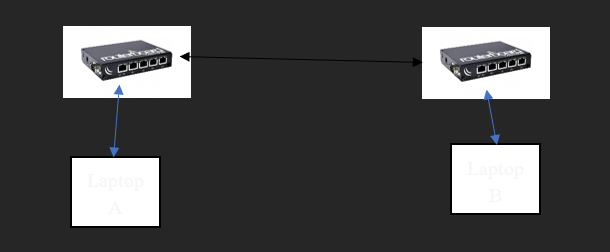
\includegraphics[width=0.7\textwidth]{image/P2/Topologi.png}    
    
    figure.1 Topologi
\end{center}


\section{Langkah Percobaan}
\begin{enumerate}
    \item 
\end{enumerate}

\section{Hasil Percobaan}


\section{Kesimpulan}


